\section{Method}
\label{sec:method}

\begin{figure*}[t]
\centering
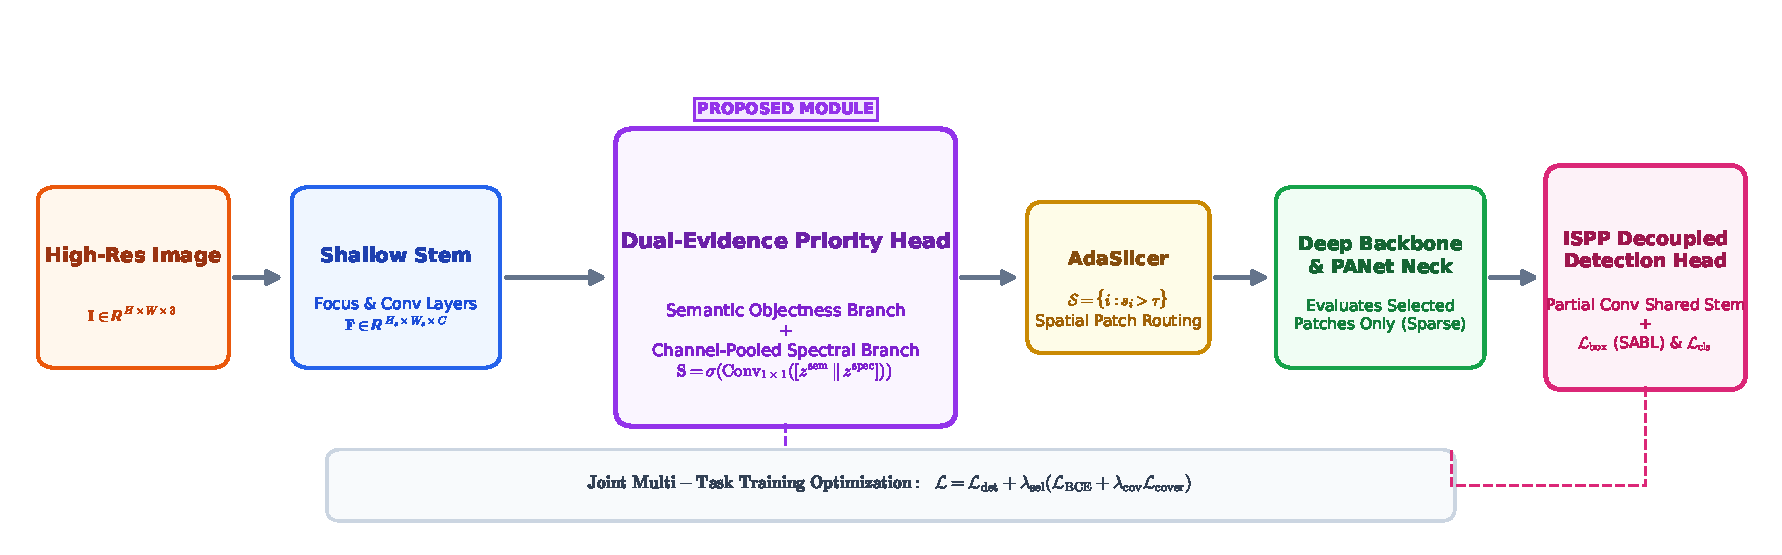
\includegraphics[width=0.92\textwidth]{hesod_overview.pdf}
\caption{DES-ESOD system overview. Grey = stock ESOD, unchanged across every
selector arm. Purple = the dual-evidence priority head (\S\ref{ssec:evidence})
that replaces ESOD's single-evidence ObjSeeker; everything downstream of the
HeatMapParser ($\mathcal{P}$) is stock, collapsed into one block since none of
it is ours.}
\label{fig:overview}
\end{figure*}

\subsection{Overview}
\label{ssec:overview}

DES-ESOD instantiates its recall-oriented, dual-evidence selector on ESOD's
patch-routing skeleton (query- and mask-level adapters for other
selective-computation backbones are outside this paper's scope). A
full-resolution image passes through a shallow stem that produces a spatial
priority heatmap. The dual-evidence head (\S\ref{ssec:evidence}) scores its
cells; ESOD's AdaSlicer thresholds the heatmap and clusters activated cells
into routed image patches. The number of resulting patches is input-dependent,
not capped. We deliberately keep this rule unchanged for the
results in \S\ref{sec:results}: it isolates the dual-evidence priority's
score construction from any change to the routing rule itself. DES-ESOD also
supports a top-$k$ heatmap-cell mode, which trades this
input-dependent activation set for an explicit cell count; that mode is evaluated separately on a
development set and is not part of the UAVDT/TinyPersonV2 results reported
here. Retained patches alone proceed through the remaining backbone/neck/head;
the rest are skipped. Section~\ref{ssec:sparsehead} records a planned, not yet
executable, within-patch sparse-head adapter.

\subsection{Dual-Evidence Priority Head}
\label{ssec:evidence}

\begin{figure}[t]
\centering
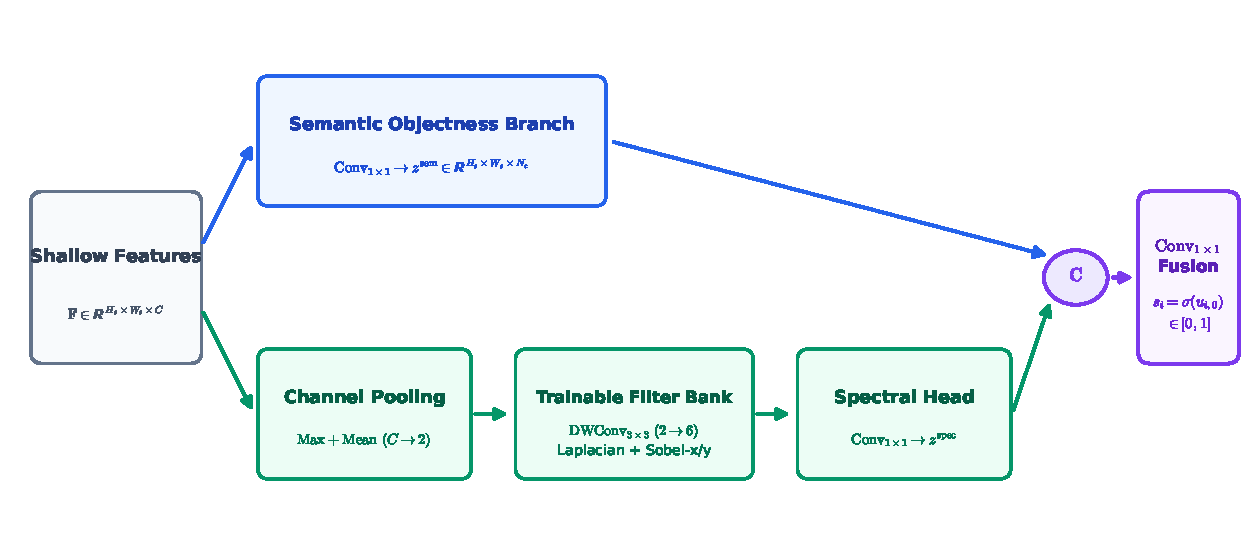
\includegraphics[width=\linewidth]{hesod_segmenter_block.pdf}
\caption{Dual-evidence priority head. Blue = semantic branch (plain
$1{\times}1$ conv). Green = channel-pooled spectral branch (no learned
backbone). \textcircled{c} = channel concatenation.}
\label{fig:evidence}
\end{figure}

For candidate cell $i$ and class channel $c$, with shared shallow feature
$f_i$, a semantic branch predicts the raw logit
$z^{\mathrm{sem}}_{i,c}=\mathrm{Conv}_{1\times1}(f_i)$, matching ESOD's
ObjSeeker interface. A parallel spectral branch first channel-pools $f_i$ to two
maps -- per-location max and mean over channels -- so the subsequent filters
operate on 2 channels regardless of backbone width, then applies a
depthwise, per-channel-group $3{\times}3$ convolution \emph{initialized} from
Laplacian and Sobel-$x$/Sobel-$y$ kernels (six output channels: one
Laplacian and two Sobel responses per pooled input); these kernels are
trainable, not fixed, so the network can move away from the classical
high-pass initialization where doing so helps routing. A $1{\times}1$
stem projects the six filter responses back to $f_i$'s channel width, and a
final $1{\times}1$ head produces the spectral logit
$z_{i,c}^{\mathrm{spec}}$ at the same per-cell resolution. This
channel-pooled design (vs.\
running the same filters on the full, un-pooled channel width) is the
low-overhead variant used throughout \S\ref{sec:results}: it is the one
structural choice that measurably improved recall on UAVDT
(\S\ref{sec:results}) without a second backbone. The two logits are
concatenated and passed through a single $1{\times}1$ fusion convolution:
\begin{equation}
u_{i,c} = \mathrm{Conv}_{1\times1}\!\left(
\left[z_{i,c}^{\mathrm{sem}} \,\|\, z_{i,c}^{\mathrm{spec}}\right]\right),
\qquad s_i=\sigma(u_{i,0}).
\label{eq:fusion}
\end{equation}
The released ESOD routing contract consumes channel~0 of the first selector
level; the current implementation preserves that contract, so $s_i$ is the
class-agnostic routing probability trained by the coverage term below, while
all fused channels retain pixelwise supervision. For a single-class dataset
this distinction disappears.
Both branches and the fusion layer add only one extra forward pass on the
already-computed shallow feature map; no second backbone is introduced,
consistent with the low-overhead constraint that spectral filtering must not
itself dominate the compute it is meant to save. Inference routing retains
$\mathcal{S} = \{i : s_i > \tau\}$, ESOD's own fixed threshold $\tau$,
unchanged (\S\ref{ssec:overview}).

\subsection{Object-Level Soft-Coverage Loss}
\label{ssec:coverage}

Let $s_i \in [0,1]$ be candidate cell $i$'s soft routing probability and
$\mathcal{N}(j)$ the rectangular set of selector-grid cells whose footprints
overlap ground-truth box $j$. The soft probability that at least one such cell
responds to $j$ is
\begin{equation}
p_j^{\mathrm{cover}} = 1 - \prod_{i \in \mathcal{N}(j)} (1 - s_i),
\end{equation}
and the coverage loss averages over all ground-truth objects,
\begin{equation}
\L_{\mathrm{cover}} = -\frac{1}{N_{\mathrm{gt}}}
\sum_{j=1}^{N_{\mathrm{gt}}} w_j \log p_j^{\mathrm{cover}},
\quad
w_j=\operatorname{clip}\!\left(\frac{4}{a_j},1,5\right),
\end{equation}
where $a_j$ is box area in selector-grid cells. Thus all objects contribute,
while objects below four grid cells receive progressively larger weight. As
any $s_i$ in $\mathcal{N}(j)$ approaches one, this term approaches zero; it
encourages but does not formally guarantee post-threshold coverage. The actual
training objective applies both pixelwise BCE and coverage supervision to the
fused selector logits:
\begin{equation}
\L_{\mathrm{sel}}=\L_{\mathrm{BCE}}(u,M;\rho{=}2)
+0.5\L_{\mathrm{cover}},\qquad
\L=\L_{\mathrm{det}}+0.2\L_{\mathrm{sel}},
\end{equation}
where $M$ denotes the selector masks and $\rho$ is the positive-class BCE
weight. There is no separate semantic-branch auxiliary loss in the current
implementation.

\subsection{Efficient Decoupled Head}
\label{ssec:head}

A YOLOv6-style decoupled head is the dominant parameter cost in an
ESOD-style detector, large enough to erase a selector's compute savings if
left unchanged. We replace it with a shared-stem decoupled head built from
ESOD-YOLO's ISPP block \cite{ESODYOLO} (channel-expand
$1{\times}1~\to$ partial $3{\times}3$ conv on a quarter of the expanded
channels $\to$ project $1{\times}1$ with residual), keeping the existing
anchor assignment, loss, and decode contract unchanged. Its contribution must
still be isolated empirically; the corresponding component-wise ablation is
retained as an experiment placeholder.

\begin{figure}[t]
\centering
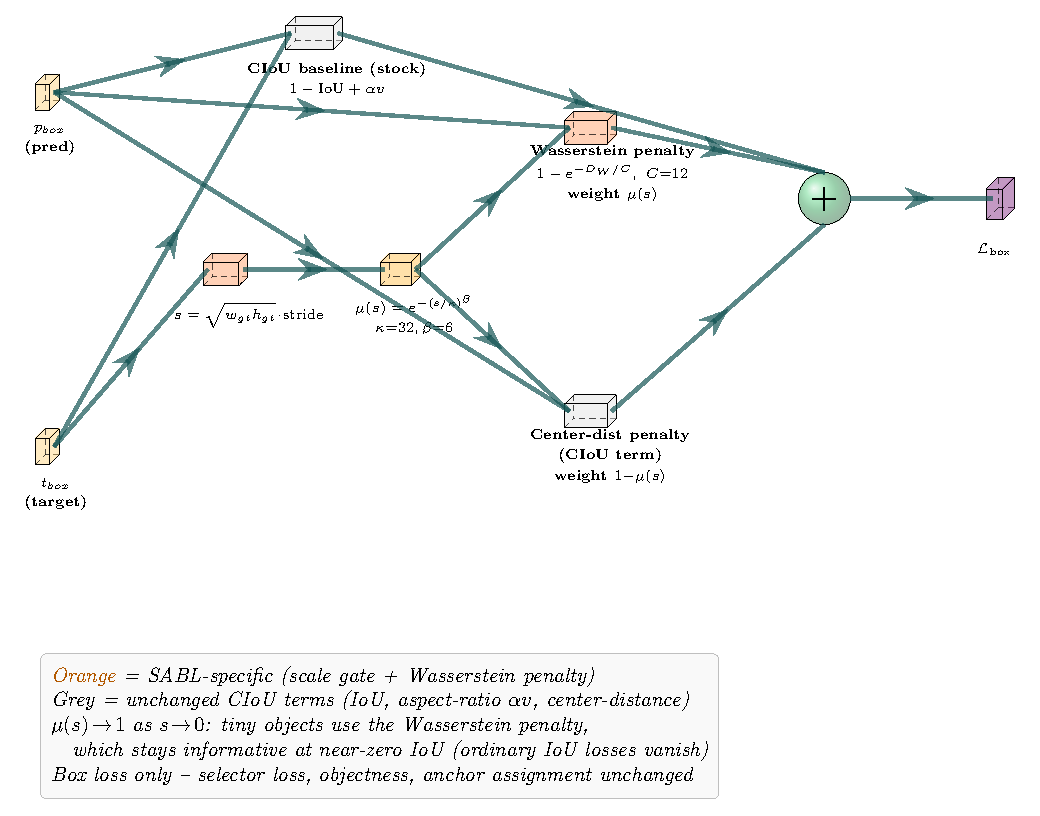
\includegraphics[width=\linewidth]{hesod_sabl_block.pdf}
\caption{SABL box loss. Orange = SABL-specific (scale gate $\mu(s)$ +
Wasserstein penalty). Grey = unchanged CIoU terms.}
\label{fig:sabl}
\end{figure}

Box regression optionally uses SSABNet's Scale-Aware Balancing Loss (SABL)
\cite{SSABNet}. Let $s=\sqrt{w_{gt}h_{gt}}$ be a matched box's geometric-mean
scale in input pixels, and $D_W$ the Wasserstein-style distance between the
predicted and target Gaussian box representations $(c_x,c_y,w/2,h/2)$, also
in input pixels. A scale-dependent weight
\begin{equation}
\mu(s) = \exp\!\left(-\left(s/\kappa\right)^{\beta}\right), \quad \kappa{=}32,\ \beta{=}6,
\end{equation}
blends a Wasserstein penalty (dominant for small $s$) with the normalized
squared center-distance penalty $\ell_{\mathrm{ctr}}$ already used by CIoU
(dominant for large $s$):
\begin{equation}
\L_{\mathrm{box}} = 1 - \mathrm{IoU} + \mu(s)\!\left(1 - e^{-D_W/C}\right) + (1-\mu(s))\,\ell_{\mathrm{ctr}} + \alpha v,
\end{equation}
with $C{=}12$ and $\alpha v$ the unchanged CIoU aspect-ratio term. As $s$
shrinks toward zero, $\mu(s)\to1$ and the loss is dominated by a distance
metric that stays informative even at near-zero IoU -- the regime ordinary
IoU-based losses give a vanishing gradient in, which is exactly where tiny
objects live. SABL is an orthogonal, opt-in treatment of the regression
target, not part of the selector claim.

\subsection{SparseHead Compatibility Placeholder}
\label{ssec:sparsehead}

\begin{figure}[t]
\centering
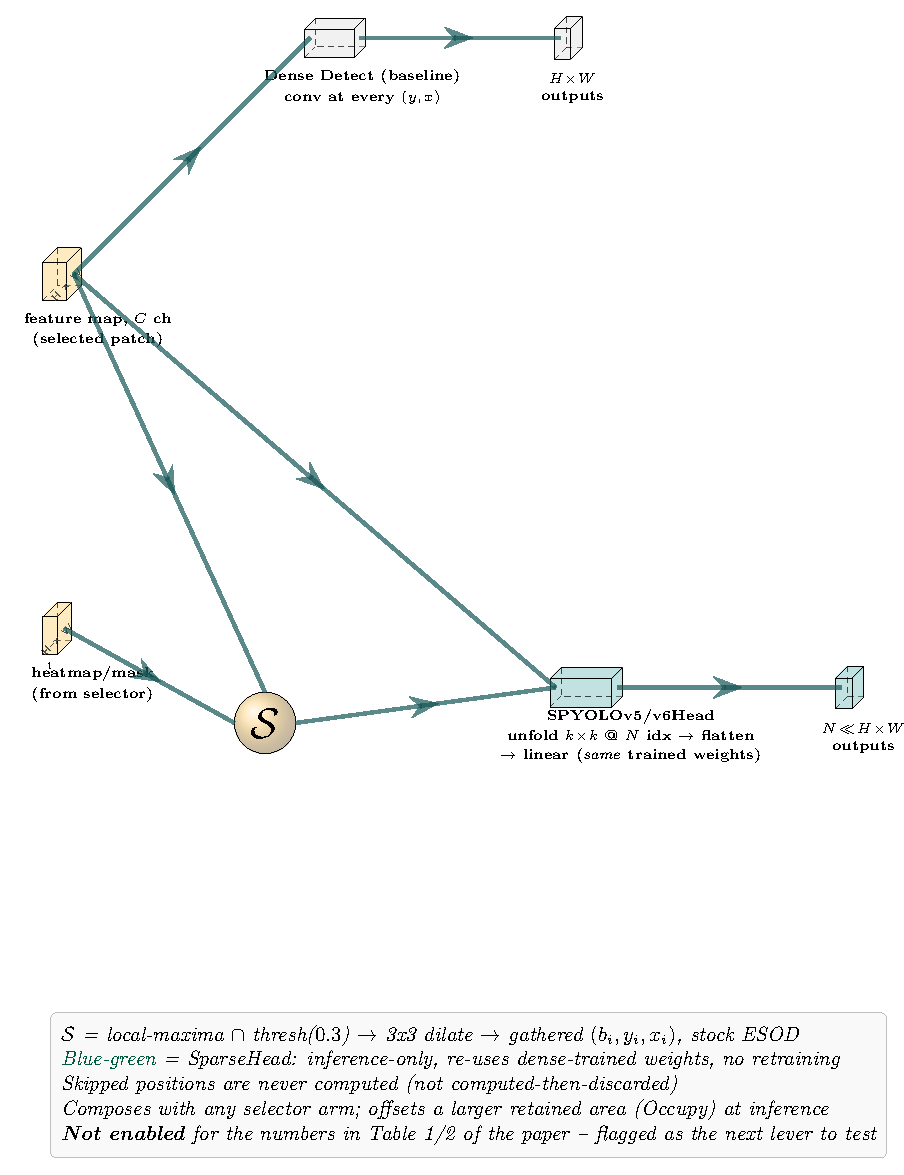
\includegraphics[width=\linewidth]{hesod_sparsehead_block.pdf}
\caption{Planned SparseHead compatibility path. $\mathcal{S}$ = local-maxima
$\cap$ threshold, dilated, as in stock ESOD. The current ISPPHead adapter is
not yet implemented.}
\label{fig:sparsehead}
\end{figure}

ESOD's SparseHead \cite{ESOD} is a natural candidate for reducing within-patch
head computation after a higher-recall selector retains more area. However,
the released conversion path currently supports ESOD's convolutional and
YOLOv6 heads only; DES-ESOD uses an ISPPHead, for which the corresponding
sparse adapter has not yet been implemented. SparseHead is therefore a code
and experiment placeholder, not part of the current executable DES-ESOD model
or any result reported below. A future adapter must map the ISPP expand,
partial-convolution, projection, and prediction layers before the
same-weight/no-retraining property can be claimed for DES-ESOD.
